

%%%% TikZ Styling and Such %%%%
    \tikzset{
        backline/.style={
            line width=3pt,color=white,shorten <=0pt,shorten >=0pt,line cap=round
        }
    }
    \tikzset{
        frontline/.style={
            color=black,shorten <=0pt,shorten >=0pt,thick,line cap=rect
        }
    }
    \tikzset{
        doublestruck/.style = {
            postaction={draw,frontline},backline
        }
    }
    \tikzset{
        vertex/.style={
            shade,
            ball color=white,
            circle,
            line width=1
        }
    }
    \tikzset{
        SolidVertex/.style={
            shade,shading=ball,
            circle,
            ball color=black!80!white,
            minimum size=3pt
        }
    }
    \tikzset{
        edges/.style={
            line width=1.5,
            every loop/.style={-},
            shorten <= 1.5pt,
            shorten >= 1.5pt,
        }
    }
    \tikzset{pics/card/.style n args={2}{
        code = {
            \draw[rounded corners=2.5pt,thick] (0,0) rectangle (2.5,3.5)
                node[pos=0.5,scale=4,font=\bfseries]{#1};
            \node[anchor=north west,scale=2] at (0,3.5) {#2};
            \node[anchor=north west,scale=2,rotate=180] at (2.5,0) {#2};
        }
    }}

%%% This file containeds TikZ Pics made by combining other pictures
    \tikzset{
    GRU/.pic={
        \draw[accent,line width=7,opacity=0.5,decorate,decoration={random steps},rounded corners] (-3,0.25) -- (3,0.25);
        \node[anchor=south] (sf) at (-2,0) {
\includegraphics[height=3cm]{images/stickfigure.png}};
        \node[anchor=south] at (0,0) {
\includegraphics[width=6cm,height=0.5cm]{images/grass.png}};
        \node[anchor=north] at (2,6) {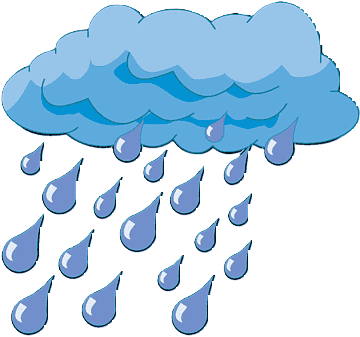
\includegraphics[height=3cm]{images/rain.png}};
        \node[anchor=south] at (sf.east) {
\includegraphics[height=2.5cm]{images/Umbrella-3-Clip-Art.png}};
    }
}

\tikzset{
    GR/.pic={
        \draw[accent,line width=7,opacity=0.5,decorate,decoration={random steps},rounded corners] (-3,0.25) -- (3,0.25);
        \node[anchor=south] (sf) at (-2,0) {
\includegraphics[height=3cm]{images/stickfigure.png}};
        \node[anchor=south] at (0,0) {
\includegraphics[width=6cm,height=0.5cm]{images/grass.png}};
        \node[anchor=north] at (2,6) {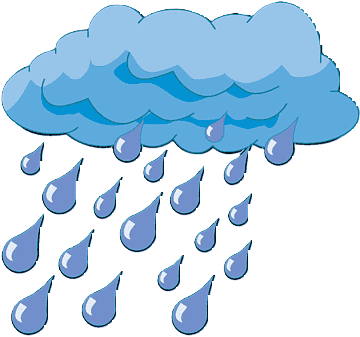
\includegraphics[height=3cm]{images/rain.png}};
    }
}

\tikzset{
    GU/.pic={
        \draw[accent,line width=7,opacity=0.5,decorate,decoration={random steps},rounded corners] (-3,0.25) -- (3,0.25);
        \node[anchor=south] (sf) at (-2,0) {
\includegraphics[height=3cm]{images/stickfigure.png}};
        \node[anchor=south] at (0,0) {
\includegraphics[width=6cm,height=0.5cm]{images/grass.png}};
        \node[anchor=south] at (sf.east) {
\includegraphics[height=2.5cm]{images/Umbrella-3-Clip-Art.png}};
    }
}

\tikzset{
    RU/.pic={
        \node[anchor=south] (sf) at (-2,0) {
\includegraphics[height=3cm]{images/stickfigure.png}};
        \node[anchor=south] at (0,0) {
\includegraphics[width=6cm,height=0.5cm]{images/grass.png}};
        \node[anchor=north] at (2,6) {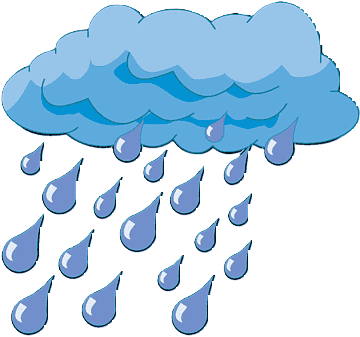
\includegraphics[height=3cm]{images/rain.png}};
        \node[anchor=south] at (sf.east) {
\includegraphics[height=2.5cm]{images/Umbrella-3-Clip-Art.png}};
    }
}

\tikzset{
    G/.pic={
        \draw[accent,line width=7,opacity=0.5,decorate,decoration={random steps},rounded corners] (-3,0.25) -- (3,0.25);
        \node[anchor=south] (sf) at (-2,0) {
\includegraphics[height=3cm]{images/stickfigure.png}};
        \node[anchor=south] at (0,0) {
\includegraphics[width=6cm,height=0.5cm]{images/grass.png}};
    }
}

\tikzset{
    R/.pic={
        \node[anchor=south] (sf) at (-2,0) {
\includegraphics[height=3cm]{images/stickfigure.png}};
        \node[anchor=south] at (0,0) {
\includegraphics[width=6cm,height=0.5cm]{images/grass.png}};
        \node[anchor=north] at (2,6) {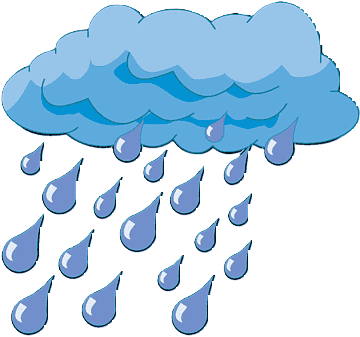
\includegraphics[height=3cm]{images/rain.png}};
    }
}

\tikzset{
    U/.pic={
        \node[anchor=south] (sf) at (-2,0) {
\includegraphics[height=3cm]{images/stickfigure.png}};
        \node[anchor=south] at (0,0) {
\includegraphics[width=6cm,height=0.5cm]{images/grass.png}};
        \node[anchor=south] at (sf.east) {
\includegraphics[height=2.5cm]{images/Umbrella-3-Clip-Art.png}};
    }
}

\tikzset{
    None/.pic={
        \node[anchor=south] (sf) at (-2,0) {
\includegraphics[height=3cm]{images/stickfigure.png}};
        \node[anchor=south] at (0,0) {
\includegraphics[width=6cm,height=0.5cm]{images/grass.png}};
    }
}

\tikzset{
    PlaneU/.pic={
        \node[anchor=south] (sf) at (-2,0) {
\includegraphics[height=3cm]{images/stickfigure.png}};
        \node[anchor=south] at (0,0) {
\includegraphics[width=6cm,height=0.5cm]{images/grass.png}};
        \node[anchor=south] at (sf.east) {
\includegraphics[height=2.5cm]{images/Umbrella-3-Clip-Art.png}};
        \node[xscale=-1,rotate=-30] at (2,4.5) {
\includegraphics[width=3cm]{images/zombie_girl_plane.png}};
    }
}

\tikzset{
    Plane/.pic={
        \node[anchor=south] (sf) at (-2,0) {
\includegraphics[height=3cm]{images/stickfigure.png}};
        \node[anchor=south] at (0,0) {
\includegraphics[width=6cm,height=0.5cm]{images/grass.png}};
        \node[xscale=-1,rotate=-30] at (2,4.5) {
\includegraphics[width=3cm]{images/zombie_girl_plane.png}};
    }
}


